\subsubsection{Qualitative evaluation on brain tumor resection dataset}

% Failures: 3 and X
% Mention the failures?

We used the \ac{BITE} dataset \cite{mercier_online_2012} to evaluate the ability of our self-supervised model to segment resection cavities on images from a different institution, modality and pathology with respect to the datasets used for quantitative evaluation.
Probabilities were thresholded at 0.5 and all but the largest binary connected component were removed.

The model successfully segmented the cavity on 11/13 images, although some contained challenging features (\figureref{fig:bite}).

\newcommand{\qualit}[1]{\includegraphics[width=0.14\linewidth]{bite/cropped/#1}}
\newcommand{\qualitfig}[1]{
    \centering
    \qualit{#1_sag}%
    \enskip
    \qualit{#1_seg_sag}%
    \quad
    \qualit{#1_cor}%
    \enskip
    \qualit{#1_seg_cor}%
    \quad
    \qualit{#1_axi}%
    \enskip
    \qualit{#1_seg_axi}
}

% https://tex.stackexchange.com/a/381477/216202
\begin{figure}[ht!]
    \centering
    \floatconts
    {fig:bite}
    {\caption{%
        Qualitative evaluation of the self-supervised model on a dataset of postoperative brain tumor \ac{T1GAD} \ac{MRI}.
        The model is robust to multiple challenging scenarios:
        low contrast between the cavity and the brain (a),
        air and \ac{CSF} within the resection cavity (b),
        highly anisotropic resolution (c),
        motion artifacts and edema (d),
        and a different modality than used for training (all).
    }}
    {
        \subfigure{%
            \label{fig:bite_low_contrast}%
            \qualitfig{2_low_contrast}
        }
        \vskip\baselineskip
        \subfigure{%
            \label{fig:bite_air}%
            \qualitfig{4_air}
        }
        \vskip\baselineskip
        \subfigure{%
            \label{fig:bite_aniso}%
            \qualitfig{5_aniso}
        }
        \vskip\baselineskip
        \subfigure{%
            \label{fig:bite_motion}%
            \qualitfig{12_motion}
        }
    }
\end{figure}



\subsubsection{Qualitative evaluation on intraoperative image}

We used our baseline model to segment the resection cavity on one intraoperative \ac{MRI} from our institution.
Despite the large domain shift between the training dataset and the intraoperative image, which includes a retracted skin flap and a missing bone flap, the model was able to correctly estimate the resection cavity segmentation, discarding other similar regions filled with \ac{CSF} or air (\figureref{fig:intra}).

\begin{figure}
    \centering
    \floatconts
    {fig:intra}
    {\caption{%
        Qualitative result on an intraoperative \ac{MRI}.
        The baseline model correctly discarded regions filled with air or \ac{CSF} that do not correspond to the resection cavity.
    }}
    {
        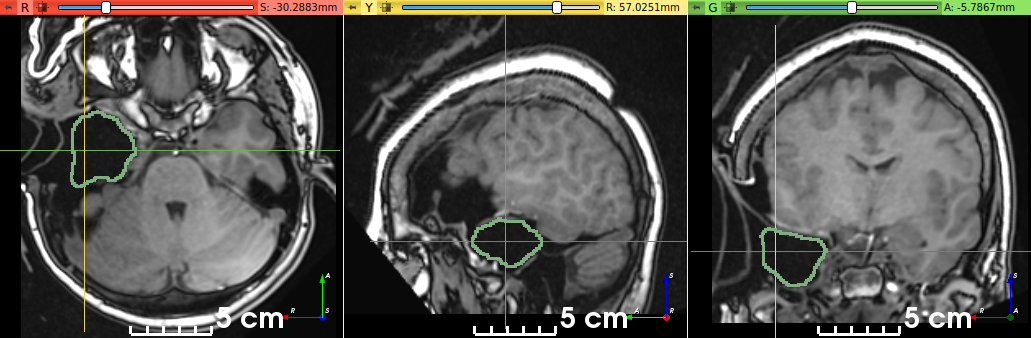
\includegraphics[trim=0 0 0 12, clip, width=\linewidth]{intra}
    }
\end{figure}